\begin{figure}[H]
\centering
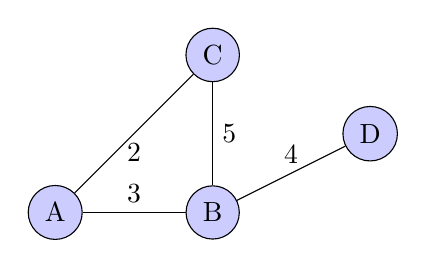
\begin{tikzpicture}
        \node[circle, draw, fill=blue!20] (A) at (0,0) {A};
        \node[circle, draw, fill=blue!20] (B) at (2,0) {B};
        \node[circle, draw, fill=blue!20] (C) at (2,2) {C};
        \node[circle, draw, fill=blue!20] (D) at (4,1) {D};
        \draw (A) -- node[above] {3} (B);
        \draw (B) -- node[right] {5} (C);
        \draw (C) -- node[below] {2} (A);
        \draw (B) -- node[above] {4} (D);
    \end{tikzpicture}
	\caption{Weighted graph example where each edge is labeled with a weight.}
    \label{fig:weighted-graph}
\end{figure}